\documentclass[11pt]{article}
\usepackage[english]{babel}
\usepackage{geometry}
\usepackage{amsmath}
\usepackage{amsthm}
\usepackage{graphicx}
\usepackage[utf8]{inputenc}

%%%%%%%% MARGIN
\geometry{verbose, letterpaper, tmargin=3cm,
  bmargin=3cm,lmargin=2.5cm,rmargin=2.5cm}

%%%%%%%% NO PARAGRAPH INDENT
% https://tex.stackexchange.com/questions/27802/set-noindent-for-entire-file
\setlength\parindent{0pt}

%%%%%%%% SUB-FIGURE PACKAGE
\usepackage{subcaption}

%%%%%%%% HYPERREF PACKAGE
\usepackage{hyperref}
\hypersetup{linkcolor=blue}
\hypersetup{citecolor=blue}
\hypersetup{urlcolor=blue}
\hypersetup{colorlinks=true}

%%%%%%%% DEFINITION AND THEOREM DEFINITIONS
\theoremstyle{definition}
\newtheorem{definition}{Definition}[section]

\theoremstyle{remark}
\newtheorem{remark}{Remark}

\theoremstyle{remark}
\newtheorem{question}{Question}

\newtheorem{theorem}{Theorem}[section]

\theoremstyle{definition}
\newtheorem{example}{Example}

%%%%%%%% MULTI-COLUMNS PACKAGE
\usepackage{multicol}

%%%%%%%% BIB-LATEX STUFF
\usepackage[style=numeric,
            bibstyle=numeric,
            citestyle=numeric,
            hyperref=true,
            backend=biber]{biblatex}
\addbibresource{ref.bib} %Put relative path to ref

%%%%%%%% DEFINITIONS
\usepackage{amssymb}
%%%% Important sets
\renewcommand{\O}{\mathbb{O}}
\newcommand{\N}{\mathbb{N}}
\newcommand{\Z}{{\mathbb{Z}}}
\newcommand{\Q}{{\mathbb{Q}}}
\newcommand{\R}{{\mathbb{R}}}

%%%% Statistics
\newcommand{\E}[1]{\mathbb{E}\left[#1 \right]}
\newcommand{\V}[1]{\mathrm{Var}\left[#1 \right]}

%%%% Lambda Calculus Symbols
\newcommand{\dneq}{\,\, \# \,\,}
\renewcommand{\S}{\pmb{\mathrm{S}}}
\newcommand{\I}{\pmb{\mathrm{I}}}
\newcommand{\K}{\pmb{\mathrm{K}}}
\newcommand{\ch}[1]{\ulcorner #1 \urcorner}

%%%% Make optional parameter
% https://tex.stackexchange.com/questions/217757/special-behavior-if-optional-argument-is-not-passed
\usepackage{xparse}
\NewDocumentCommand{\cx}{o}{
  \IfNoValueTF{#1}
  {\left[\quad\right]}
  {\left[\, #1 \,\right]}
}

%%%%%%%% LOGIC TREES
\usepackage{prftree}

%%%%%%%% SPLIT EQUATIONS
% https://tex.stackexchange.com/questions/51682/is-it-possible-to-pagebreak-aligned-equations
\allowdisplaybreaks

%%%%%%%% TO USE H SPECIFIER
\usepackage{float}

%%%%%%%% TO USE SHORT COMMANDS FOR VECTOR LINES
\usepackage{esvect}

%%%%%%%% START DOCUMENT

\title{$\lambda$-Calculus}
\author{Juan Sebasti\'an C\'ardenas-Rodríguez \\
        \scalebox{0.7}{Mathematical Engineering, Universidad EAFIT}}
\date{\today}


\begin{document}
\maketitle
Notes based on \parencite{barendregt2004}.

\section{$\pmb{\lambda}$ Theory}

\subsection{Basic Definitions}
\begin{definition}
  The set of $\lambda$-terms $\Lambda$ is defined recursively as:
  \begin{itemize}
    \item $x \in \Lambda$
    \item $M \in \Lambda$ then $\lambda x.M \in \Lambda$
    \item $M, N \in \Lambda$ then $M\,N \in \Lambda$
  \end{itemize}
\end{definition}

With $x$ being a variable. The following rules are used for the convertibility
relationship, denoted by $=$, defined in the set $\Lambda$. \\

\textbf{$\pmb{\beta}$-conversion}
%
\begin{equation*}
  \prftree{(\lambda x.M)N = M\left[x := N\right]}
\end{equation*}
%
\textbf{Equality axioms}
%
\begin{equation*}
  \begin{array}{ccc}
    \prftree{M = M} \qquad & \prftree{M = N}{N = M} \qquad
    & \prftree{M = N}{N = L}{M = L}
  \end{array}
\end{equation*}
%
\textbf{Compatibility Rules}
%
\begin{equation*}
  \begin{array}{ccc}
    \prftree{M = N}{ML = NL} \qquad & \prftree{M = N}{LM = LN} \qquad &
    \prftree[r]{$\xi$-rule}{M = N}{\lambda x.M = \lambda x.N}
  \end{array}
\end{equation*}
%
Which, the terms of the new defined $\pmb{\lambda}$ Theory are the elements of
$\Lambda$, with the formulae being of the type $M = N$, with $M, N \in \Lambda$.
It is important to notice that, although the symbol for convertibility is
defined, a notation for writing that a $\lambda$-term is not convertible to
another is not defined.

Furthermore, a $\lambda$-term is considered to be close if it happens that it
does not have any free variables. It is also called a combinator. The set of all
combinators is noted by $\Lambda^0$

\begin{definition}
  The set of sub-terms of a $\lambda$-term $M$ is denoted by Sub$(M)$ and is
  defined by:
  \begin{enumerate}
    \item Sub$(x) = \{x\}$
    \item Sub$(\lambda x.M) = \text{Sub}(M)\cup\{\lambda x.M\}$
    \item Sub$(M\,N) = \text{Sub}(M) \cup \text{Sub}(N)$
  \end{enumerate}
  Hence, it can be said that a $\lambda$-term $M$ is subset of another term $N$
  if it occurs that $M \in \text{Sub}(N)$.
\end{definition}

\begin{definition}
  A $\lambda$-term $M$ is in normal form if $M$ does not have a sub-term of the
  form $(\lambda x.R)S$. Furthermore, it has a normal form if it happens that
  $M = N$ and $N$ is a $\lambda$- term that is in normal form.
\end{definition}

Some important lambda terms are defined by:
%
\begin{equation*}
  \begin{split}
    &\I \equiv \lambda x. x \quad \K \equiv \lambda xy. x \\
    &\S \equiv \lambda xyz. xz(yz)
  \end{split}
\end{equation*}

\subsection{Incompatibility}

\begin{definition}
  Two $\lambda$-terms $M, N$ are incompatible if it happens that the
  $\pmb{\lambda}$-theory with the addition to the axiom $M = N$ leads to an
  inconsistent theory. It is noted as $M \dneq N$
\end{definition}

When we deduce a convertibility $L = R$ of two lambda terms, using the extended
theory (adding the axiom $M=N$) we noted as
$\pmb{\lambda} + M = N \vdash L = R$. Furthermore, two terms are incompatible if
their normal form are different.

With this fact, then it can be proved that lambda calculus is Hilbert-Post
complete. Hence, we obtain the following theorem:
\begin{theorem}
  Suppose $M, N$ have a normal form. Then either $\pmb{\lambda} \vdash M=N$ or,
  exclusively, $M \dneq N$.
\end{theorem}

\subsection{Exercises First Class}
\begin{question}
  Show that the following terms have a normal form:
  \begin{enumerate}
  \item $(\lambda y.yyyy)((\lambda ab.a)\I(\S\S))$
  \item $(\lambda yz.zy)((\lambda x.xxx)(\lambda x.xxx))(\lambda w. \pmb{I})$
  \item $\S\S\S\S\S\S\S$
  \end{enumerate}
\end{question}
\begin{proof}
  \begin{enumerate}
    \item Let's reduce that term to a normal form term:
          %
          \begin{align*}
            (\lambda y.yyy)((\lambda ab.a)\I(\S\S)) &= (\lambda y.yyy)((\lambda b.\I)
                                                      (\S\S)) \\
                                                    &= (\lambda y.yyy)(\I) \\
                                                    &= \I\I\I \\
                                                    & = \I
          \end{align*}
          %
    \item Let's reduce that term to a normal form term:
          \begin{align*}
            (\lambda yz.zy)((\lambda x.xxx)(\lambda x.xxx))(\lambda w. \I)
            &= (\lambda w. \I)((\lambda x.xxx)(\lambda x.xxx)) \quad \\
            &= \I
          \end{align*}

    \item Let's reduce that term to a normal form term:
          \begin{align*}
            \S\S\S\S\S\S\S &= \S\S(\S\S)\S\S\S \\
                           &= \S\S(\S\S\S)\S\S \\
                           &= \S\S(\S\S\S\S)\S \\
                           &= \S\S(\S\S\S\S\S) \\
                           &= \lambda z_0. \S z_0(\S\S\S\S\S z_0) \\
                           &= \lambda z_0z_1.z_0z_1(\S\S\S\S\S z_0z_1) \\
                           &= \lambda z_0z_1.z_0z_1(\S\S(\S\S)z_0z_1) \\
                           &= \lambda z_0z_1.z_0z_1(\S z_0(\S\S z_0)z_1) \\
                           &= \lambda z_0z_1. z_0z_1(z_0z_1(\S\S z_0z_1)) \\
                           &= \lambda z_0z_1. z_0z_1(z_0z_1(\S z_1(z_0z_1))) \\
                           &= \lambda z_0z_1. z_0z_1(z_0z_1(\lambda z_2. z_1z_2(z_0z_1z_2)))
          \end{align*}
  \end{enumerate}
\end{proof}

\begin{question}
  Show that:
  \begin{itemize}
    \item $\I \dneq \K$
    \item $\I \dneq \S$
    \item $xy \dneq xx$
  \end{itemize}

  \begin{proof}
    \begin{itemize}
      \item Let's show that they are incompatible. Then, let's add as axiom that
            $\I = \K$.
            %
            \begin{align*}
              \I &= \K \\
              \I XY &= \K XY \\
              XY &= X \\
                 &\text{Making } X = \I \text{ and } Y
                   \in \Lambda \text{ arbitrary, then:} \\
              \I Y &= \I \\
              Y &= \I
            \end{align*}
            %
            Therefore, it occurs that $\pmb{\lambda} + \I = \K \vdash Y = \I$,
            for any lambda term. Hence, we arrived at an inconsistent theory.
    \end{itemize}
  \end{proof}
\end{question}

\subsection{Exponentiation}
\begin{definition}
  Let $F, M \in \Lambda$. Then:
  \begin{itemize}
    \item $F^0M \equiv M \quad F^{n+1}M \equiv F(F^nM)$
    \item $FM^{\sim 0} \equiv F \quad FM^{\sim n + 1} \equiv FM^{\sim n}M $
  \end{itemize}
\end{definition}

\subsection{Contexts}
\begin{definition}
  A \textit{context} $C\cx$ is a term with some holes in it. More formally:
  \begin{enumerate}
    \item $x$ is a context, with $x$ being a random variable.
    \item $\cx$ is a context.
    \item If $C_1\cx$ and $C_2\cx$ are contexts, then so are $C_1\cx C_2\cx$ and
          $\lambda x. C_1\cx$.
  \end{enumerate}
  Furthermore, if $C\cx$ is a context and $M \in \Lambda$, then $C\cx[M]$
  denotes the result of placing $M$ in the holes of $C\cx$. This is beneficial
  as free variables in $M$ may be bounded when placed.
\end{definition}

\begin{remark}
  When it is said that $C\cx$ is a context, it is formally noted by
  $C\cx \in \Lambda$.
\end{remark}

\subsection{Definable Functions}
\begin{definition}
  A Church numeral is the representation of natural numbers in lambda calculus.
  They are defined easily as:
  %
  \begin{equation*}
    \ch{n} \equiv \lambda fx. f^nx
  \end{equation*}
  %
  With this one can defined $\lambda$-definable functions (or recursive
  functions as expressed in Turing Machines). These are functions
  $f: \N^k \rightarrow \N$ that it happens that it exists a $F \in \Lambda^0$
  that happens:
  %
  \begin{equation*}
    F \, \ch{n_1} \, \ch{n_2} \, \dots \, \ch{n_k} = \ch{f\, n_1\, n_2\, \dots \,n_k}
  \end{equation*}
\end{definition}

\subsection{Exercises Second Class}
\begin{question}
  Let $C\cx \in \Lambda$. Then:
  %
  \begin{equation*}
    N = N' \rightarrow C\cx[N] = C\cx[N']
  \end{equation*}
\end{question}

\begin{proof}
  Let's prove by induction on the structure of contexts.
  \begin{itemize}
    \item If $C\cx = x$, then it is obtained that:
          %
          \begin{align*}
            &C\cx[N] = x \quad C\cx[N'] = x \\
            &C\cx[N] = C\cx[N']
          \end{align*}

  \item If $C\cx = \cx$, then it is obtained that:
          %
          \begin{align*}
            &C\cx[N] = N \quad C\cx[N'] = N' \\
            &C\cx[N] = C\cx[N'] \quad \text{ because } N = N'
          \end{align*}

    \item If $C_1\cx, \, C_2\cx \in \Lambda$ for which it occurs that
          $C_1\cx[N] = C_1\cx[N']$ and $C_2\cx[N] = C_2\cx[N']$, then let's see
          that is also happens for $C\cx \equiv C_1\cx C_2\cx$.
          %
          \begin{align*}
            C_1\cx[N] &= C_1\cx[N'] \\
            C_1\cx[N]C_2\cx[N] &= C_1\cx[N']C_2\cx[N] \\
                      &\text{Also} \\
            C_2\cx[N] &= C_2\cx[N'] \\
            C_1\cx[N']C_2\cx[N] &= C_1\cx[N']C_2\cx[N'] \\
                      &\text{Hence} \\
            C_1\cx[N]C_2\cx[N] &= C_1\cx[N']C_2\cx[N'] \\
            C\cx[N] &= C\cx[N']
          \end{align*}
    \item If $C_1\cx \in \Lambda$ for which it occurs that
          $C_1\cx[N] = C_1\cx[N']$, then let's show that it happens to
          $C\cx = \lambda x. C_1\cx$
          %
          \begin{align*}
            C_1\cx[N] &= C_1\cx[N'] \\
            \lambda x. C_1\cx[N] &= \lambda x. C_1\cx[N'] \\
            C\cx[N] &= C\cx[N']
          \end{align*}
  \end{itemize}
\end{proof}

\begin{question}
  Let $X\equiv\S\I$ show that $XXXX = X(X(XX))$. Does $X^nX = XX^{\sim n}$ hold
  $\forall n \in \N$?
  \begin{proof}
    It is important to notice that:
    %
    \begin{align*}
      &X \equiv \S\I = \lambda yz. \I z(yz) \text{ Therefore } \\
      &XMN = \I N (M N) = N (M N)
    \end{align*}
    %
    Therefore
    %
    \begin{equation*}
      XXXX = X(XX)X = X (XXX) = X(X(XX))
    \end{equation*}
    %
    In these manner, let's prove by induction that it holds for all $n \in \N$.
    \begin{itemize}
      \item $X^0X \equiv X = X$ and $XX^{\sim 0} \equiv X = X$, therefore
            $X^0X = XX^{\sim 0}$.
      \item Let's suppose that for some $n \ge 0$ it occurs that
            $X^nX = XX^{\sim n}$. Let's show that
            $X^{n + 1}X = XX^{\sim n + 1}$.
            %
            \begin{align*}
              XX^{\sim n + 1} &= XX^{\sim n}X \\
                              &= X^nXX \\
            \end{align*}
            %
            Let's show, then, that $\forall n \in \N$, it occurs that
            $X^nXX = X(X^nX)$.
            \begin{itemize}
              \item $X^0XX = XX$ and $X(X^0X) = XX$. Hence, for $n=0$ is true.
              \item Let's suppose that for some $n \ge 0$ it occurs that
                    $X^nXX = X(X^nX)$. Let's show it is true for $n + 1$.
                    \begin{align*}
                      X^{n+1}XX &= X(X^nX)X \\
                                &= X(X^nXX) \\
                                &= X(X(X^nX)) \\
                                &= X(X^{n + 1}X)
                    \end{align*}
            \end{itemize}
            Hence, using the previous proof then we continue in the following
            manner:
            \begin{align*}
              XX^{\sim n + 1} &= X^nXX \\
                              &= X(X^nX) \\
                              &=X^{n + 1}X
            \end{align*}
    \end{itemize}
  \end{proof}
\end{question}

\begin{question}
  Suppose a symbol of the $\lambda$-calculus alphabet is always 0.5 cm wide.
  Write down a $\lambda$-term with length less than 20 cm having a normal form
  with length at least $10^{10^{10}}$ light-year. The of speed light is
  $c = 3 \cdot 10^{10} \text{cm}/\text{s}$
\end{question}
\begin{proof}
  It is clear that we can only use less than 40 symbols. In these manner, let's
  calculate how many symbols does the normal form of the lambda-term need to
  have:
  \begin{equation*}
    10^{10^{10}} \cdot 3 \cdot 10^{10} \cdot 2 \cdot 3600 \cdot 24 \cdot 365.25 =
    1.893456 \cdot 10^{118} < 10^{120}
  \end{equation*}
  In these manner, we need to construct a $\lambda$-term which when reduced to
  normal form it contains more than $10^{120}$ symbols.

  A way to solve this exercise is to construct a $\lambda$-definable function,
  such that for a small input grows rapidly. The good thing about $\lambda$-
  definable functions is that their normal form is equal to the representation
  of their church numeral.

  Hence, a function such as the \textcite{ackermann1928} function. This function
  is defined as:
  %
  \begin{alignat*}{3}
    &A : &&\N^2 \rightarrow \N &&\\
    &A &&0 \,\, m &&= m + 1 \\
    &A &&(n + 1)\, 0 &&= A \, n \, 1 \\
    &A &&(n + 1) \, (m + 1) &&= A \, n \, (A \, (n + 1)\, m)
  \end{alignat*}
  %
  This function is really helpful, as $A \, 4 \, 2$ is a number of 19729 digits.
  Furthermore, in \parencite{goldberg2000} it is shown that the function is
  $\lambda$-definable by this lambda term,
  %
  \begin{equation*}
    \pmb{\mathrm{Ack}} = \lambda p. p (\lambda aq. a(q a (\lambda fx. fx)))(\lambda nfx. f(n f x))
  \end{equation*}
\end{proof}

\begin{definition}
  The result of substituting $N$ for the free occurrences of $x$ in $M$
  ($M[x := N]$) is defined as follows:
  \begin{itemize}
    \item $x[x := N] \equiv N$
    \item $y[x:=N] \equiv y$
    \item $(\lambda y.M)[x := N] \equiv \lambda y. (M[x := N])$
    \item $(M_1M_2)[x := N] \equiv (M_1[x := N]) (M_2[x := N])$
  \end{itemize}
\end{definition}

\subsection{Fixed Point Theorem}
\begin{theorem}
  For all $F \in \Lambda$ it exists a $X \in \Lambda$ such that $FX = X$. This
  is called the fixed point theorem.
\end{theorem}
\begin{proof}
  Let $W = \lambda x. F(xx)$ and $X = WW$. Then:
  %
  \begin{align*}
    X &= WW \\
      &= (\lambda x. F(xx))W \\
      &= F(WW) \\
      &= FX
  \end{align*}
\end{proof}

\subsection{Exercises Third Class}
\begin{question}
  \label{q:blackbox}
  Show that $\nexists F \,\,\forall MN \,\,F(MN) = M$. (\textit{Hint}: Show that
  $F(xy) \dneq x$)
\end{question}
\begin{proof}
  Let's see that $F(xy) \dneq x$ for a $F \in \Lambda$.
  %
  \begin{align*}
    F(xy) &= x \\
    (\lambda zw. w) F(xy) &= (\lambda zw. w) x\\
    xy &= \lambda w.w
  \end{align*}
  %
  Therefore, we obtained that $\pmb{\lambda} + F(xy)=x \vdash xy = \I$, which is
  not true as they are both in normal form and syntactically different. In this
  manner, it exists two lambda terms for which it does not exist an $F$ such
  that $F(MN) = M$, $M = x$, $N = y$.

  In this manner, as it does not exist for one case then it does not exists for
  all cases.
\end{proof}

\begin{question}
  Show that $\exists M \,\, \forall N \,\, MN = MM$. (\textit{Hint}: Use the
  fixed point theorem)
\end{question}
\begin{proof}
  Let $W=\lambda xy. xx(xx)$. Then, let $M = WW$. Hence:
  %
  \begin{align*}
    MN &= WWN \\
       &= (\lambda xy. xx(xx))WN \\
       &= WW(WW) \\
       &= MM
  \end{align*}
\end{proof}

\begin{question}
  Show that $(\lambda y. (\lambda x. M))N = \lambda x. ((\lambda y.M)N)$
\end{question}
\begin{proof}
  Let's apply the definition of substituting:
  %
  \begin{align*}
    (\lambda y. (\lambda x. M)) N &= (\lambda x. M)\cx[y := N] \\
                                  &\equiv \lambda x. (M\cx[y := N]) \\
                                  &\text{On the other hand} \\
    \lambda x. ((\lambda y. M)N) &= \lambda x. (M\cx[y := N])
  \end{align*}
  %
  Hence, by transitivity we obtain that:
  %
  \begin{equation*}
    (\lambda y. (\lambda x. M)) N = \lambda x. ((\lambda y. M)N)
  \end{equation*}
\end{proof}

\subsection{Black Box}
Some more popular combinators are:
%
\begin{align*}
  \pmb{\mathrm{B}} &= \lambda fgx.f(gx) \\
  \pmb{\mathrm{B}'} &= \lambda fgx.g(fx) \\
  \K^* &= \lambda xy. y \\
  \pmb{\mathrm{W}} &= \lambda fx.fxx
\end{align*}
%
As a previous exercise proves, it is impossible to read inside $\lambda$-terms
(Question \ref{q:blackbox}). Therefore, one could say that $\lambda$-terms are
black boxes. In the exercises section of this class, one can find some
$\lambda$-terms that cannot be constructed due to this property.

\subsection{Exercises Fourth Class}
\begin{question}
  Prove that the following $F \in \Lambda$ do not exist for all $M \in \Lambda$.
  \begin{itemize}
    \item
          \begin{equation*}
            FM =
            \begin{cases}
              \ch{1}, &\quad \text{If } M \text{ is a variable} \\
              \ch{2}, &\quad \text{If } M \text{ is an application} \\
              \ch{3}, &\quad \text{If } M \text{ is a
              } \lambda \text{-abstraction}
            \end{cases}
          \end{equation*}
    \item
          \begin{equation*}
            GM =
            \begin{cases}
              \ch{1}, &\quad \text{If } M \text{ is in } \beta \text{-normal form} \\
              \ch{0}, &\quad \text{otherwise} \\
            \end{cases}
          \end{equation*}
    \item
          \begin{equation*}
            HM = \ch{n}, \quad \text{where } \ch{n}
            \text{ is the number of abstractions of } M
          \end{equation*}
  \end{itemize}
\end{question}
\begin{proof}
  Let's prove each of the literals.
  \begin{itemize}
    \item Let's add to the theory the axiom. Hence, it exists an $F$ such that
          has the mentioned behavior. In this manner, it is easy to notice that:
          %
          \begin{align*}
            F((\lambda x. x)y) &= \ch{2} \text{ Furthermore}\\
            F((\lambda x. x)y) &= Fy \text{ But }\\
            Fy &= \ch{1} \text{ Hence, by transitivity }\\
            \ch{2} &= \ch{1}
          \end{align*}
          %
          Which is not true as both are in normal form and are syntactically
          different.

    \item Let's add to the theory the axiom. Hence, it exists an $G$ such that
          has the mentioned behavior. In this manner, it is easy to notice that:
          %
          \begin{align*}
            G((\lambda x. x)y) &= \ch{0} \text{ Furthermore}\\
            G((\lambda x. x)y) &= Gy \text{ But }\\
            Gy &= \ch{1} \text{ Hence, by transitivity }\\
            \ch{2} &= \ch{1}
          \end{align*}
          %
          Which is not true as both are in normal form and are syntactically
          different.

    \item Let's add to the theory the axiom. Hence, it exists an $F$ such that
          has the mentioned behavior. In this manner, it is easy to notice that:
          %
          \begin{align*}
            H((\lambda x. x)y) &= \ch{1} \text{ Furthermore}\\
            H((\lambda x. x)y) &= Hy \text{ But }\\
            Hy &= \ch{0} \text{ Hence, by transitivity }\\
            \ch{1} &= \ch{0}
          \end{align*}
          %
          Which is not true as both are in normal form and are syntactically
          different.
  \end{itemize}
\end{proof}

\begin{question}
  Construct an $M \in \Lambda^0$, such that $M = M\S$.
\end{question}
\begin{proof}
  Let $W = \lambda x. xx\S$, and $M = WW$. Then:
  %
  \begin{align*}
    M &= WW \\
      &= (\lambda x. xx\S)W \\
      &= WW\S \\
      &= M\S
  \end{align*}
\end{proof}

\begin{question}
  Construct an $M \in \Lambda^0$, such that $M\I\S\S = M\S$.
\end{question}
\begin{proof}
  Let $W = \lambda xyz.xx$ and $M = WW$. Then:
  \begin{align*}
    M\I\S\S &= (\lambda xyz. xx)W\I\S\S \\
            &= WW\S \\
            &= M\S
  \end{align*}
\end{proof}

\newpage
\section{Reduction}
For this section, let's define the combinator:
%
\begin{equation*}
  \Omega \equiv (\lambda x. xx)(\lambda x. xx)
\end{equation*}

\subsection{Basic Definitions}
The binary relation $\beta$ on $\Lambda$ is defined by:
\begin{equation*}
  \beta = \{((\lambda x.M)N, M\cx[x := N]) \mid M, N \in \Lambda\}
\end{equation*}

\begin{definition}
  A binary relation $\pmb{R}$ on $\Lambda$ is compatible iff for every
  $L \in \Lambda$:
  %
  \begin{align*}
    (M, N) \in \pmb{R} \Rightarrow& (LM, LN) \in \pmb{R} \\
                                  &(ML, NL) \in \pmb{R} \\
                                  &(\lambda x.M, \lambda x.N) \in \pmb{R}
  \end{align*}
\end{definition}
Furthermore a $P$ closure of a relation $\pmb{R}$ is when the relationship is
modified in order to satisfy property $P$. Hence:

\begin{definition}
  The binary relation \textbf{one step $\beta$-reduction} on $\Lambda$, denoted
  by $\rightarrow_\beta$, is the compatible closure of $\beta$. Hence, it can be
  defined inductively:
  %
  \begin{equation*}
    \prftree{(M, N) \in \beta}{M \rightarrow_\beta N}
  \end{equation*}
  %
  \begin{equation*}
    \prftree{M \rightarrow_\beta N}{L \in \Lambda}{LM \rightarrow_\beta LN} \qquad
    \prftree{M \rightarrow_\beta N}{L \in \Lambda}{ML \rightarrow_\beta NL} \qquad
    \prftree{M \rightarrow_\beta N}{\lambda x.M \rightarrow_\beta \lambda x.N}
  \end{equation*}
    %
  If $M \rightarrow_\beta N$ it is said that $M$ $\beta$-reduces in one-step to
  $N$.
\end{definition}

\begin{definition}
  The binary relation \textbf{$\beta$-reduction} on $\Lambda$, denoted by
  $\rightarrow_\beta$, is the reflexive and transitive closure of $\beta$.
  Hence, it can be defined inductively:
  %
  \begin{equation*}
    \prftree{M \rightarrow_\beta N}{M \twoheadrightarrow_\beta N}
  \end{equation*}
  %
  \begin{equation*}
    \prftree{M \twoheadrightarrow_\beta M} \qquad
    \prftree{M \twoheadrightarrow_\beta N}{N \twoheadrightarrow_\beta L}
    {M \twoheadrightarrow_\beta L}
  \end{equation*}
  %
  If $M \twoheadrightarrow_\beta N$ it is said $M$ $\beta$-reduces to $N$.
\end{definition}

\begin{definition}
  Finally, $=_\beta$ the equivalence relation generated by
  $\twoheadrightarrow_\beta$. Hence, it can be defined inductively:
  %
  \begin{equation*}
    \prftree{M \twoheadrightarrow_\beta N}{M =_\beta N}
  \end{equation*}
  %
  \begin{equation*}
    \prftree{M =_\beta N}{N =_\beta M} \qquad
    \prftree{M =_\beta N}{N =_\beta L}{M =_\beta L}
  \end{equation*}
  %
  If $M =_\beta N$ then it is said that $M$ is $\beta$-convertible to $N$.
\end{definition}

With this relationship, one could then define what $\beta$-redex and
$\beta$-normal is.

\begin{definition}
  A $\beta$-redex is a term $M$ such that $(M, N) \in R$ for some term $N$. In
  this case $N$ is called an $\beta$-contractum.

  A term is in $\beta$-normal form if it does not contain any $\beta$-redex.

  Furthermore, if $M$ is in $\beta$-normal form then:
  \begin{itemize}
    \item For no $N$, it happens that $M \rightarrow_\beta N$.
    \item If $M \twoheadrightarrow_\beta N$, then $M \equiv N$.
  \end{itemize}
\end{definition}


\subsection{Reduction Graphs}
With this relationships, one could then define a reduction graph for a term $M$,
noted by $G_\beta(M)$. That graph, is defined as a set of vertices and a
relationship between does vertices call edges. Hence, the vertices of a
reduction graph are:
%
\begin{equation*}
  \{N \in \Lambda \mid M \twoheadrightarrow_\beta N\}
\end{equation*}
%
with the edges being $M \rightarrow_\beta N$.

\begin{example}
  Let's see some examples.
  \begin{itemize}
    \item $G_\beta(WWW)$ with $W = \lambda xy. xyy$. It is clear that
          $WM = \lambda y. Wyy$. The reduction graph is:
          \begin{figure}[h]
            \centering
            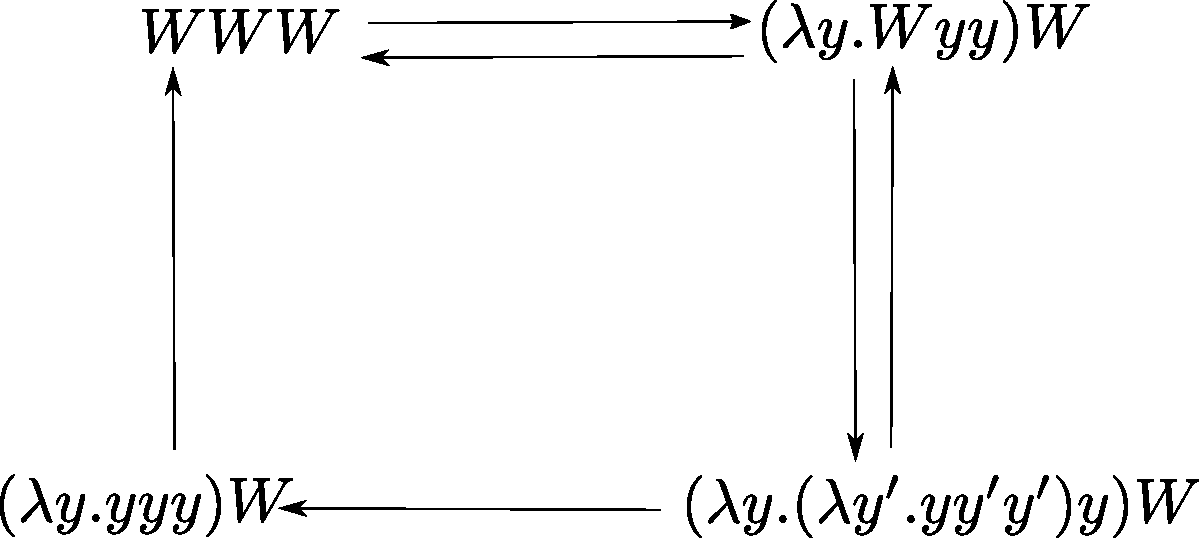
\includegraphics[scale=0.4]{../graphs/example-graph-1.pdf}
          \end{figure}

    \item $G_\beta(MM)$ with $M = \lambda x. (\lambda y.yy)x$.
          \begin{figure}[h]
            \centering
            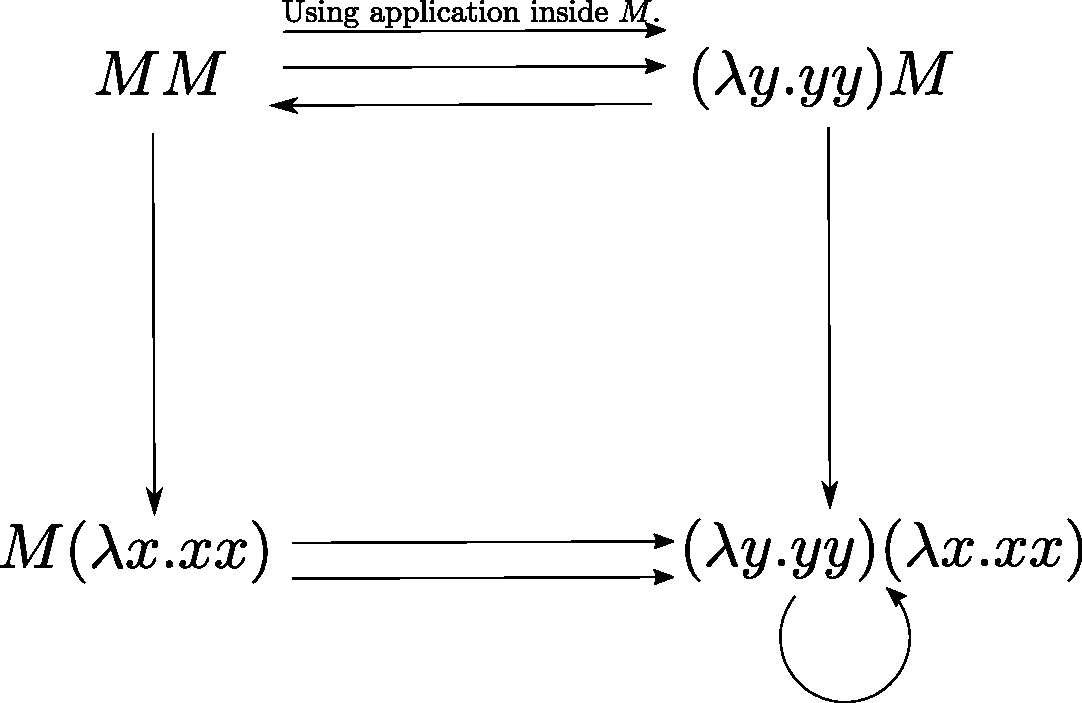
\includegraphics[scale=0.4]{../graphs/example-graph-2.pdf}
          \end{figure}

    \item $G_\beta(\Omega)$
          \begin{figure}[H]
            \centering 
\includegraphics[scale=0.4]{../graphs/example-omega.pdf}
          \end{figure}
  \end{itemize}
  Normally, the $\beta$-reduction graphs do not have the terms as the node and
  have a single point in substitution of it. In this notes, the term is written
  to help understanding.
\end{example}

\subsection{Exercises Fifth Class}
\begin{question}
  It happens that $M =_\beta N \iff \pmb{\lambda} \vdash M = N$. Prove the
  $\Rightarrow$ of the previous statement.
\end{question}
\begin{proof}
  Let's prove it by induction in the structure of each of the relationships.
  \begin{itemize}
    \item Let's prove it on $\rightarrow_\beta$.
          \begin{itemize}
            \item If $(M, N) \in \beta$, hence it is clear that $M$ has the form
                  of $(\lambda x. M')N'$. Furthermore, $N$ has the form
                  $M'[x := N']$. Furthermore:
                  %
                  \begin{align*}
                    M &\equiv (\lambda x. M')N' \\
                      &= M'[x := N'] \text{ by } \beta\text{-conversion} \\
                      &= N
                  \end{align*}
                  %
                  Hence, $\pmb{\lambda} \vdash M = N$

            \item Let's suppose that if
                  $M \rightarrow_\beta N \Rightarrow \pmb{\lambda} \vdash M = N$
                  for some terms $M, N$ then $\pmb{\lambda} \vdash LM = LN$, for
                  a term $L$. Let's show that to
                  $\pmb{\lambda} \vdash LM = LN \wedge ML = NL \wedge (\lambda x. M) = (\lambda x. N)$.
                  %
                  \begin{align*}
                    M \rightarrow_\beta N &\Rightarrow M = N
                                            \text{ Inductive hypotheses}\\
                    M &= N\\
                    LM &= LN \text{ by a compatibility rule} \\
                    M &= N\\
                    ML &= NL \text{ by a compatibility rule} \\
                    M &= N\\
                    \lambda x.M &= \lambda x. N \text{ by a compatibility rule} \\
                  \end{align*}
                  %
                  Hence,
                  $M \rightarrow_\beta N \Rightarrow \pmb{\lambda} \vdash M = N$
          \end{itemize}

    \item Let's prove it on $\twoheadrightarrow_\beta$.
          \begin{itemize}
            \item If $M \rightarrow_\beta N$, then
                  $M \twoheadrightarrow_\beta N$. Furthermore, as
                  $M \rightarrow_\beta N$ then $M = N$ by the previous proof.

            \item It is clear that $M \twoheadrightarrow_\beta M$. Furthermore,
                  as the convertibility is reflexive, it is also true that
                  $M = M$.

            \item Let's suppose that $M \twoheadrightarrow_\beta N$ and
                  $N \twoheadrightarrow_\beta L$ satisfy that $M = N$ and
                  $N = L$. Let's see that $M \twoheadrightarrow_\beta L$
                  satisfies that $M = L$. We have that:
                  %
                  \begin{equation*}
                    \prftree{M = N}{N = L}{M = L}
                  \end{equation*}
                  Hence, we obtain that $M = L$. In conclusion, if
                  $M \twoheadrightarrow_\beta N \Rightarrow M = N$
          \end{itemize}

    \item Let's prove it on $=_\beta$
          \begin{itemize}
            \item If $M \twoheadrightarrow_\beta N$, then $M =_\beta N$.
                  Furthermore, as $M \twoheadrightarrow_\beta N$ then $M = N$ by
                  the previous proof.

            \item Let's suppose that $M \twoheadrightarrow_\beta N$ satisfies
                  that $M = N$. Let's see it also is satisfied for
                  $N \twoheadrightarrow_\beta M$. We have that:
                  %
                  \begin{equation*}
                    \prftree{M = N}{N = M}
                  \end{equation*}
                  %
                  Hence, it is obtained that $N = M$.

            \item Let's suppose that $M =_\beta N$ and $N =_\beta L$ satisfy
                  that $M = N$ and $N = L$. Let's see that $M =_\beta L$
                  satisfies that $M = L$. We have that:
                  %
                  \begin{equation*}
                    \prftree{M = N}{N = L}{M = L}
                  \end{equation*}
                  %
                  Hence, we obtain that $M = L$.
          \end{itemize}
  \end{itemize}
  In conclusion, if $M =_\beta N \Rightarrow M = N$
\end{proof}

\begin{question}
  Draw $G(M)$ with
  \begin{itemize}
    \item $M \equiv (\lambda x. \I xx)(\lambda x. \I xx)$. Let's say
          $W = \lambda x. \I xx$
          \begin{figure}[H]
            \centering
            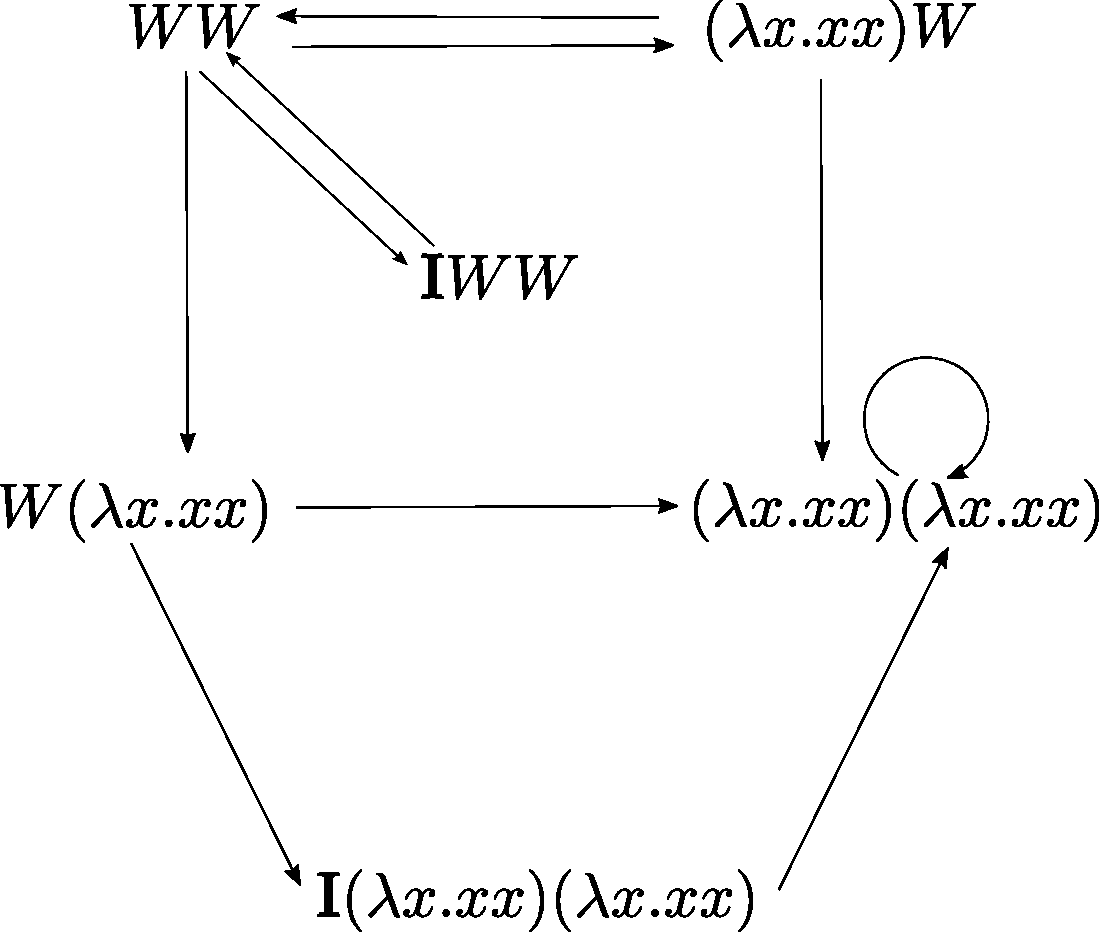
\includegraphics[scale=0.4]{../graphs/exercise-3-5-1-i.pdf}
          \end{figure}

    \item $M \equiv (\lambda x. \I (xx))(\lambda x. \I (xx))$. Let
          $W = \lambda x. \I (xx)$.
          \begin{figure}[H]
            \centering
            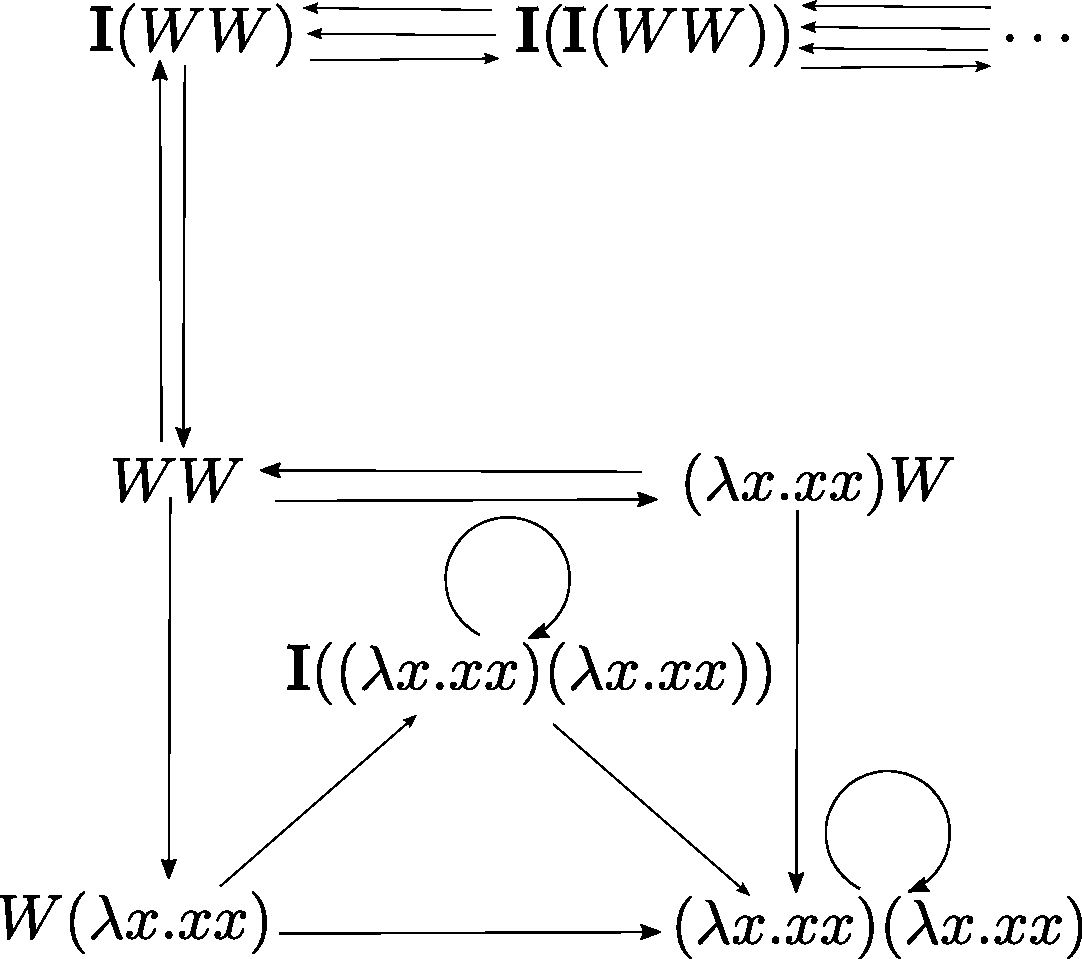
\includegraphics[scale=0.4]{../graphs/exercise-3-5-1-ii.pdf}
          \end{figure}
  \end{itemize}
\end{question}

\begin{question}
  Find terms with the following lambda term:
  \begin{itemize}
    \item $G_\beta(M) =$
          \begin{figure}[H]
            \centering
            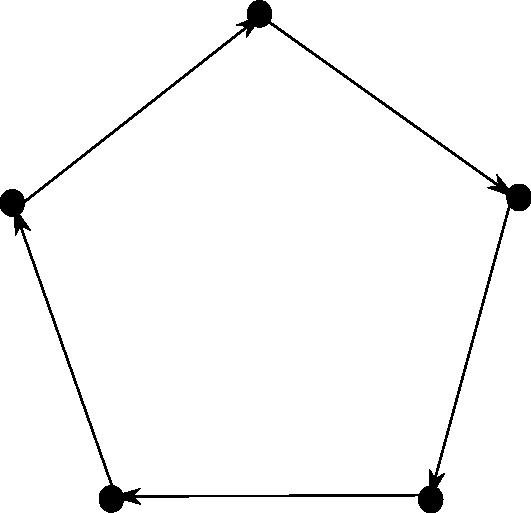
\includegraphics[scale=0.5]{../graphs/exercise-3-5-2-i.pdf}
          \end{figure}
          Generalize to $n$ vertices.

    \item $G_\beta(M) = $
          \begin{figure}[H]
            \centering
            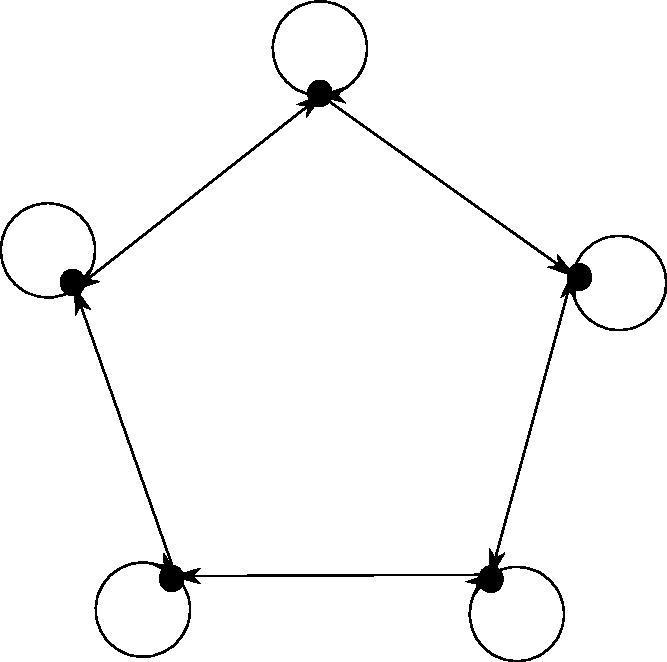
\includegraphics[scale=0.5]{../graphs/exercise-3-5-2-ii.pdf}
          \end{figure}

    \item $G_\beta(M) = $
          \begin{figure}[H]
            \centering
            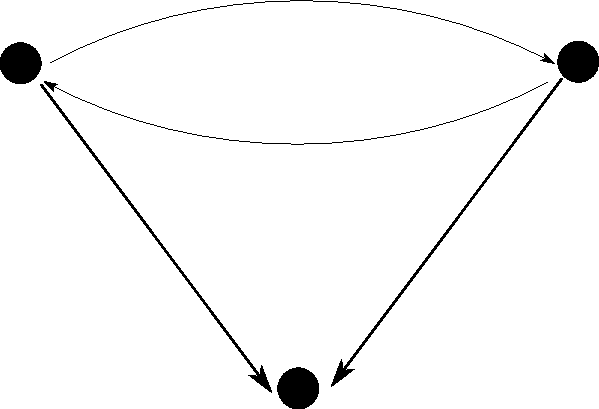
\includegraphics[scale=0.5]{../graphs/exercise-3-5-2-iii-1.pdf}
          \end{figure}

    \item $G_\beta(M) = $
          \begin{figure}[H]
            \centering
            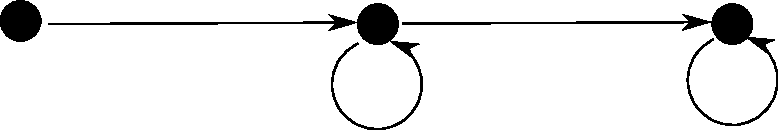
\includegraphics[scale=0.5]{../graphs/exercise-3-5-2-iii-2.pdf}
          \end{figure}

    \item $G_\beta(M) = $
          \begin{figure}[H]
            \centering
            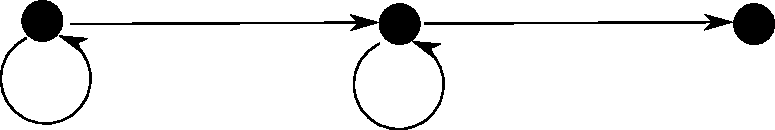
\includegraphics[scale=0.5]{../graphs/exercise-3-5-2-iii-3.pdf}
          \end{figure}
  \end{itemize}
\end{question}

\begin{proof}
  Let's show each of terms that satisfy that property.
  \begin{itemize}
    \item Let's define the term $R = \lambda abcdf. fabcdf$ and therefore
          $M = R\I\I\I\I R$. Let's see it's relationships:
          %
          \begin{align*}
            M &\twoheadrightarrow_\beta (\lambda bcdf. f\I bcdf)\I\I\I R \\
              &\twoheadrightarrow_\beta (\lambda cdf. f\I\I df)\I\I R \\
              &\twoheadrightarrow_\beta (\lambda df. f\I\I\I df)\I R \\
              &\twoheadrightarrow_\beta (\lambda f. f\I\I\I\I f) R \\
              &\twoheadrightarrow_\beta R\I\I\I\I R \equiv M
          \end{align*}
          %
          It is clear that the previous term satisfies the reduction graph
          proposed. To follow a similar idea to the term selected before, let's
          define the variables $\vv{x_n} \equiv y_0 \ldots y_{n-1}$ and define
          the sequence of lambda terms as:
          %
          \begin{align*}
            R_0 \equiv y_0 &\quad R_{n+1} \equiv \lambda \vv{x_{n+1}}. (y_{n} \vv{x_{n+1}}) \\
            M_0 \equiv R_0 &\quad M_{n+1} \equiv R_{n+1} \vv{x_n} R_{n+1}
          \end{align*}
          %
          Let's proof that this is a generalization to each $n$.
          \begin{itemize}
            \item For $n = 0$, it is clear that $M_0$ is in normal form. Hence,
                  the graph would be just a node.
            \item For $n = n' + 1$, let's define
                  $\vv{x_n}^i \equiv y_i \ldots y_{n-1}$ for $i < n$. Hence, we
                  would obtain a graph like this:
                  \begin{figure}[H]
                    \centering
                    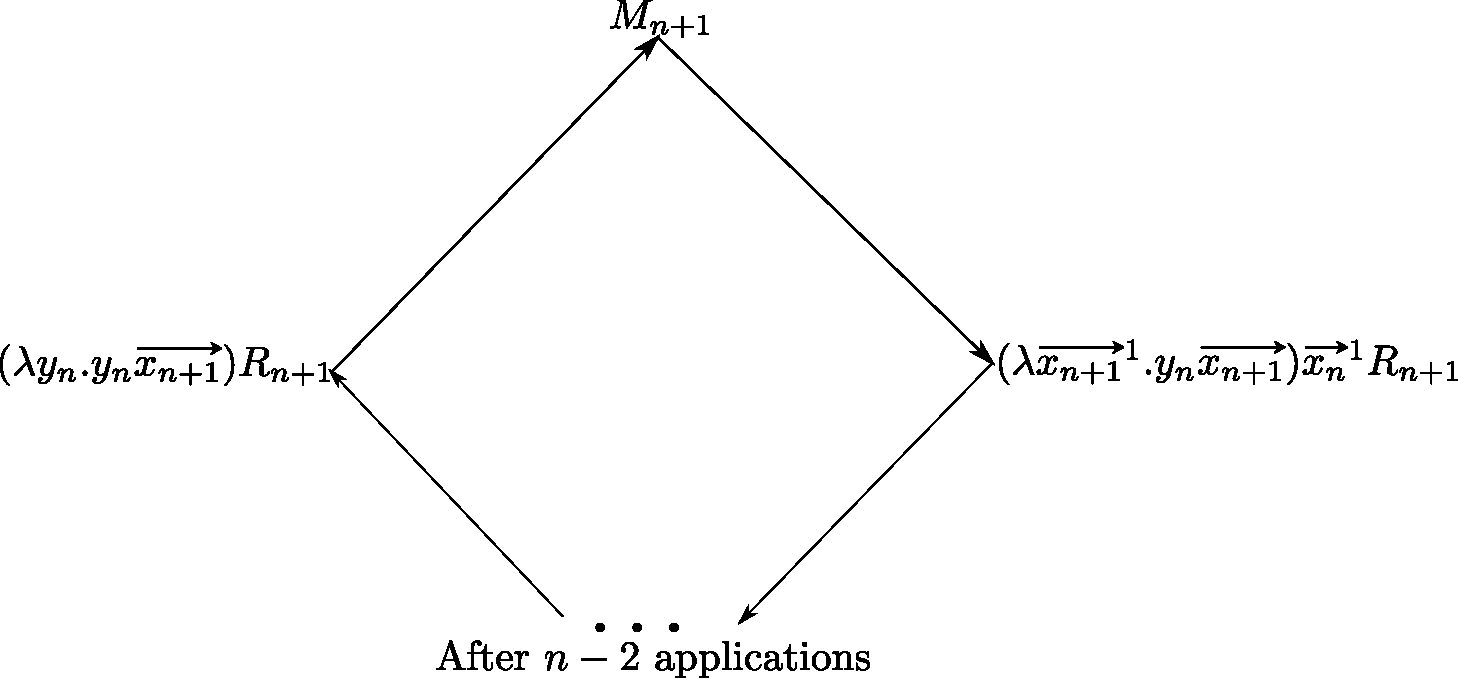
\includegraphics[scale=0.5]{../graphs/exercise-3-5-2-i-n.pdf}
                  \end{figure}
          \end{itemize}

    \item It is easy to see that the term $M = \Omega (R \I\I\I\I R)$, with
          $R = \lambda abcdf. fabcdf$.

    \item For this graph is easily seen that the term $M = \K^*(WxW)$, with
          $W = \lambda xy. yxy$, satisfies it. This is happens because:
          %
          \begin{alignat*}{2}
            M &\twoheadrightarrow_\beta \K^*((\lambda y. yxy)W)
            &&\twoheadrightarrow_\beta \K^* (WxW) \equiv M \\
            &\twoheadrightarrow_\beta \I &&\twoheadrightarrow_\beta \I
          \end{alignat*}

    \item The term $M = (\lambda xy. xx) (\lambda z. zz) y$ satisfies the
          proposed reduction graph. Remember that
          $\Omega \twoheadrightarrow_\beta \Omega$ (not by transitivity). Hence:
          %
          \begin{align*}
            M \twoheadrightarrow_\beta (\lambda y. \Omega) y
            & \twoheadrightarrow_\beta \Omega
              \twoheadrightarrow_\beta \Omega\\
            &\twoheadrightarrow_\beta (\lambda y. \Omega) y
          \end{align*}

    \item The term $M = (\lambda y. y\Omega)(\lambda x. y)$ satisfies the
          reduction graph as:
          %
          \begin{alignat*}{2}
            M &\twoheadrightarrow_\beta (\lambda x. y)\Omega
            &&\twoheadrightarrow_\beta y \\
            &\twoheadrightarrow_\beta (\lambda y. y\Omega)(\lambda x.y) \equiv M
            &&\twoheadrightarrow_\beta (\lambda x. y)\Omega
          \end{alignat*}
  \end{itemize}
\end{proof}

\subsection{Exercises Sixth Class}
\begin{question}
  $\beta-\mathrm{SN}(M)$ implies $G_\beta(M)$ is finite and $M$ has a
  $\beta$-nf, but not conversely.
\end{question}

\begin{question}
  Show that:
  \begin{enumerate}
    \item If $G_1$ and $G_2$ are the $\beta$-graphs of some term, then so is
          their cartesian product.
    \item If $G$ is the $\beta$-graph of a term, then so is $G \mapsto K_1$ (add
          one point that is below each point of $G$).
  \end{enumerate}
\end{question}

\begin{question}
  Let $R$ be a notion of reduction. Show that if $R-\mathrm{SN}(M)$ and each
  $R$-redex has only finitely many contracta, then $G_R(M)$ is finite.
\end{question}

\printbibliography
\end{document}
